\section{Mi primera aplicación}
  Ahora veremos cómo crear una aplicación con \textit{IntelliJ}, será algo muy simple, pero nos
  servirá como base para comenzar el segundo arco de este libro.

  Lo primero que necesitamos es entender la estructura del proyecto.
  En la carpeta del proyecto debieran haber 3 elementos: el archivo \texttt{intellij-basics.iml}, y 
  las carpetas \texttt{.idea} y \texttt{src}.
  Su utilidad es:
  \begin{itemize}
    \item \texttt{.idea}: contiene la configuración de IntelliJ.
    \item \texttt{src}: contiene el código fuente de nuestra aplicación.
    \item \texttt{intellij-basics.iml}: es el archivo de configuración del proyecto.
  \end{itemize}

  En la mayoría de los casos, no nos van a interesar mucho los archivos de configuración, así que
  interactuaremos solamente con el directorio \texttt{src}.

  \subsection{Paquetes}
    De la misma forma en que un computador se organiza en carpetas, un proyecto se organiza en 
    paquetes.

    El principal objetivo de los paquetes es darle organización a nuestro código, porque, al igual 
    que tener una carpeta repleta de archivos (te estoy mirando a ti que tienes el escritorio 
    tapizado en íconos), tener todo el código de nuestra aplicación en una carpeta (o en el mismo 
    archivo \texttt{D:}) es barbarie.

    La gracia de usar paquetes en vez de simplemente carpetas es que podemos incorporar la lógica de
    los paquetes en nuestro código.
    Además, si se utilizan correctamente podemos evitar gran parte de los problemas que podrían
    surgir al momento de interactuar con librerías externas.
    
    \textit{Kotlin} (al igual que \textit{Java} y \textit{Scala}) permiten organizar nuestro código 
    en paquetes, mientras que otros lenguajes como \textit{Python} y \textit{C++} 
    no.\footnote{En lugar de paquetes \textit{Python} provee módulos y \textit{C++} tiene 
    \textit{namespaces}, ambas cumplen los mismos objetivos que los paquetes, pero se utilizan de 
    forma distinta. 
    Es importante informarse de esas diferencias cuando están aprendiendo un nuevo lenguaje.}
    El estándar para nombrar paquetes es el mismo para \textit{Java}, \textit{Kotlin} y 
    \textit{Scala}: 
    \begin{itemize}
      \item El nombre del paquete debe ser único (se recomienda usar el dominio de la empresa o 
        persona que lo creó).
      \item El nombre del paquete debe ser escrito en minúsculas.
      \item El nombre del paquete no debe incluir guiones bajos (\texttt{\_}).
      \item El nombre del paquete puede incluir guiones (\texttt{-}), pero no se recomienda.
    \end{itemize}

    Veamos algunos ejemplos:
    
    \begin{kotlin}
      package cl.ravenhill.intellij.basics; // Bien
      package cl.ravenhill.intelliJBasics; // Mal, el nombre no debe incluir mayúsculas
      package cl.ravenhill.intellij_basics; // Mal, el nombre no debe incluir guiones bajos
      package cl.ravenhill.intellij-basics; // Permitido, pero no recomendado
    \end{kotlin}

    Busquemos la carpeta \texttt{src/main/kotlin} y creemos un paquete llamado 
    \url{cl.ravenhill.intellij.basics} haciendo click derecho sobre la carpeta \texttt{kotlin} y 
    seleccionando \textit{New} \texttt{->} \textit{Package}.

    \begin{figure}[ht!]
      \centering
      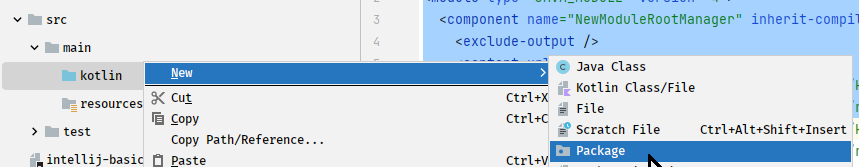
\includegraphics[width=0.8\textwidth]{img/Por_algo_se_empieza/idea64_new_package.png}
      \caption{Creando un nuevo paquete}
      \label{fig:idea64_new_package}
    \end{figure}

    Es importante acostumbrarse a crear paquetes para organizar el código por dos razones:
    \begin{itemize}
      \item Siempre que se trabaje con librerías externas, es muy probable que se encuentren con 
        paquetes que no son de su propiedad, y que no pueden modificar.
      \item Cuando una aplicación crece, los paquetes nos permiten organizar el código de forma 
        lógica.
    \end{itemize}

  \subsection{Mi primer \textit{Kotlin}}
    Ahora que ya sabemos cómo crear paquetes, vamos a crear nuestro primer archivo \textit{Kotlin}.
    Para ello, haremos click derecho sobre el paquete que acabamos de crear y seleccionaremos
    \textit{New} \texttt{->} \textit{Kotlin File/Class} (\cref{fig:idea64_new_kotlin_file}), y en
    el dialogo que aparece crearemos un archivo \texttt{InteractiveFibonacciCalculator} 
    (\cref{fig:idea64_new_kotlin_file_dialog}).

    \begin{figure}[ht!]
      \centering
      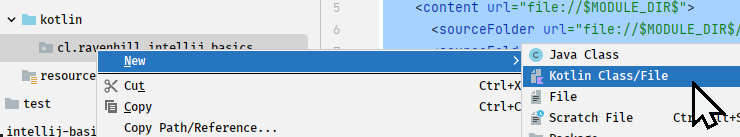
\includegraphics[width=0.8\textwidth]{img/Por_algo_se_empieza/idea64_new_kotlin_file.png}
      \caption{Creando un nuevo archivo \textit{Kotlin}}
      \label{fig:idea64_new_kotlin_file}
    \end{figure}

    \begin{figure}[H]
      \centering
      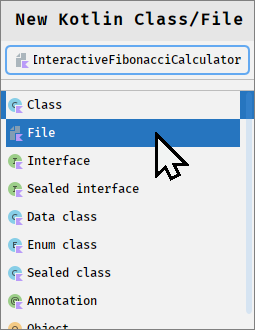
\includegraphics{img/Por_algo_se_empieza/idea64_new_kotlin_file_dialog.png}
      \caption{Creando un nuevo archivo \textit{Kotlin}}
      \label{fig:idea64_new_kotlin_file_dialog}
    \end{figure}

    Esto creará un archivo \texttt{InteractiveFibonacciCalculator.kt} en la carpeta
    \url{src/main/kotlin/cl/ravenhill/intellij/basics}.
    Noten que el nombre del archivo utiliza \textit{PascalCase}.

    Ahora vamos a escribir el código que calcula la sucesión de Fibonacci de forma interactiva.
    Lo primero que debemos conocer aquí es la función \texttt{main}.
    Esta función es el punto de entrada, es decir, es la función que se ejecuta cuando se corre el
    programa.

    Existe más de una forma de escribir la función \texttt{main} en \textit{Kotlin}, pero 
    utilizaremos la más simple, que es definir una función \texttt{main(): Unit}.
    Podemos partir con algo como:

    \begin{kotlin}
      package cl.ravenhill.intellij.basics

      fun main() {
        println("Welcome to the Fibonacci Calculator!")
      }
    \end{kotlin}

    ¡Y listo! 
    Tenemos nuestra primera aplicación en \textit{Kotlin}.
    Para ejecutarla, buscaremos el botón 
